%%%%%%%%%%%%%%%%%%%%%%%%%%%%%%%%%%%%%%
%% Frame
%%%%%%%%%%%%%%%%%%%%%%%%%%%%%%%%%%%%%%

\begin{frame}[t]
\frametitle{Numerical Results}
\framesubtitle{~~}  %% needed for proper positioning of the logo ...

We tested the DFR and circulant/Toeplitz sensing matrices on a small example
test image. The image was a Modified Shepp-Logan phantom which was $128\times 128$
pixels.

\begin{figure}[h!]
  \centering
	\caption{Modified Shepp-Logan phantom reconstructed using a circulant matrix with RPMS restriction}
    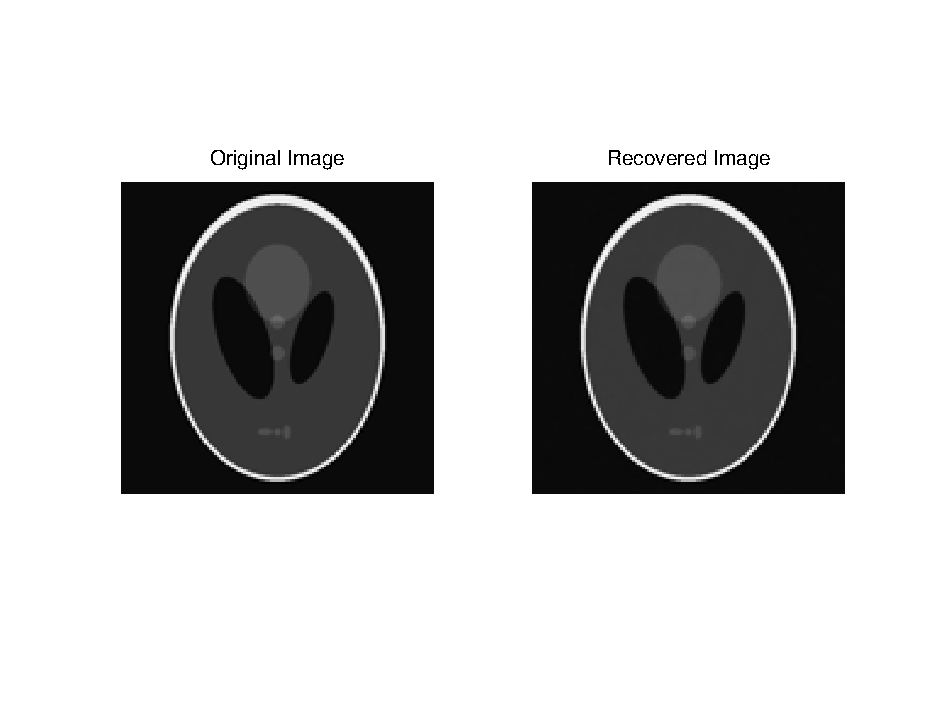
\includegraphics[width=0.6\textwidth]{figs/rpms.pdf}
\end{figure}

\end{frame}


%%%%%%%%%%%%%%%%%%%%%%%%%%%%%%%%%%%%%%
%% Frame
%%%%%%%%%%%%%%%%%%%%%%%%%%%%%%%%%%%%%%

\begin{frame}[t]
\frametitle{Matrix Type and Error}
\framesubtitle{~~}  %% needed for proper positioning of the logo ...




\begin{table}[h]
\begin{tabular}{lll|lllll}
	\textbf{Matrix Type}       & \textbf{Input Randomizer} & \textbf{Output Randomizer} & \textbf{Error} & \textbf{Time} & \\ \hline
	\multirow{2}{*}{Circulant} & \multirow{2}{*}{N/A}      & Sub                   & 0.0156         & 4.97s         & \\
	                           &                           & RPMS                  & 0.0159         & 7.80s         & \\
\end{tabular}
\end{table}

\begin{table}[h]
\begin{tabular}{lll|lllll}
	\textbf{Matrix Type}      & \textbf{Input Randomizer} & \textbf{Output Randomizer} & \textbf{Error} & \textbf{Time} & \\ \hline
	\multirow{2}{*}{Toeplitz} & \multirow{2}{*}{N/A}      & Sub                   & 0.0193         & 25.9s         & \\
	                          &                           & RPMS                  & 0.0170         & 16.9s         & \\
\end{tabular}
\end{table}

\end{frame}


%%%%%%%%%%%%%%%%%%%%%%%%%%%%%%%%%%%%%%
%% Frame
%%%%%%%%%%%%%%%%%%%%%%%%%%%%%%%%%%%%%%

\begin{frame}[t]
\frametitle{Matrix Type and Error}
\framesubtitle{~~}  %% needed for proper positioning of the logo ...


\begin{table}[h]
\begin{tabular}{lll|lllll}
	\textbf{Matrix Type}     & \textbf{Input Randomizer} & \textbf{Output Randomizer} & \textbf{Error} & \textbf{Time } & \\ \hline
	\multirow{4}{*}{Fourier} & \multirow{2}{*}{Local}    & Sub                        & 0.0183         & 7.89s          & \\
	                         &                           & RPMS                       & 0.0517         & 14.0s          & \\
	                         & \multirow{2}{*}{Global}   & Sub                        & 0.0166         & 4.98s          & \\
	                         &                           & RPMS                       & 0.0529         & 14.1s          & \\
\end{tabular}
\end{table}

\begin{table}[h]
\begin{tabular}{lll|lllll}
	\textbf{Matrix Type}      & \textbf{Input Randomizer} & \textbf{Output Randomizer} & \textbf{Error} & \textbf{Time } & \\ \hline
	\multirow{4}{*}{Hadamard} & \multirow{2}{*}{Local}    & Sub                        & 0.0167         & 552s           & \\
	                          &                           & RPMS                       & 0.0153         & 752s           & \\
	                          & \multirow{2}{*}{Global}   & Sub                        & 0.0157         & 544s           & \\
	                          &                           & RPMS                       & 0.0137         & 782s           & \\
\end{tabular}
\end{table}


\end{frame}

%%%%%%%%%%%%%%%%%%%%%%%%%%%%%%%%%%%%%%
%% Frame
%%%%%%%%%%%%%%%%%%%%%%%%%%%%%%%%%%%%%%

\begin{frame}[t]
\frametitle{Timing}
\framesubtitle{~~}  %% needed for proper positioning of the logo ...

For these timing results, we use the same image as before, but half the size, as the 
Gaussian (dense, unstructured) matrix was too large.


\begin{table}[h]
\begin{tabular}{l|lllllll}
	\textbf{Matrix Type} & Gaussian & Circulant & Toeplitz & Fourier & Hadamard \\ \hline
	\textbf{Time}        & 12.2s    & 1.65s     & 4.24s    & 1.50s   & 102s*    \\
\end{tabular}
\end{table}
* The fast Walsh-Hadamard transform in \textsc{Matlab} is written in \textsc{Matlab} and is slow.


\end{frame}
